\section{Stratification and Safety}
\label{sec:safety}
In the previous section we demonstrated that \slang can capture
intuitive notions of persistence and mutability of state via a
stylized use of Datalog.  However, the alert reader will note that
even very simple \slang programs make for unusual Datalog: among other
concerns, persistence rules produce derivations for an infinite number
of values of the time suffix.  Traditional Datalog interpreters, which
work against static databases, would attempt to enumerate these
values, making this approach impractical.

However, in the context of distributed systems and networks, the need
for non-terminating ``services'' or ``protocols'' is very common.  In
this section we show that expressing distributed systems properties
such as persistence and mutable state in logic does not require
dispensing with familiar notions of safety and stratification: we take
traditional notions of acceptable Datalog programs, and extend them in
a way that admits sensible non-terminating programs.



\subsection{Stratification in {\large{\bf\slang}}}
\label{sec:strat}
We first turn our attention to the semantics of
programs with negation.  As we will see, the inclusion of time enables
programs' local stratification, and the existence of a unique perfect model
that corresponds to intuition. \wrm{reword}

%``source of monotonicity''  a unique perfect model

%semantics in some surprising cases, and enables purely syntactic monotonicity
%checks for a broad class of temporal programs.

%%\paa{notes}

%%this section has become cluttered, but for me the main results are the following:

%%\begin{enumerate}
%%\item Negation-, aggregation- and choice-free \lang programs have a unique minimal model (pure Datalog)
%%\item stratifiable \lang programs have a unique minimal model (again, Datalog, but we need to show that the restrictions and syntactic transformations
%%cannot introduce a cycle or add a negative edge to an existing cycle.)
%%\item \emph{temporally stratified} \lang programs (w/o choice) force any cycles with negation to involve an inductive edge, forcing an ordering on the evaluation.
%%we can show that in all such cases, the corresponding datalog program is modularly stratified (insofar as \emph{successor} is considered to be ``completely
%%evaluated" in a lower module.)  since modularly stratified programs have a unique stable model, so do any temporally stratified \lang programs.
%%\end{enumerate}

\begin{lemma} \label{lemma:no-neg-unique}
%
A \slang program without negation 
%%and aggregation 
has a unique minimal model.
%
\end{lemma}

\begin{proof} 
%
A \slang program without negation 
%%and aggregation 
is a pure Datalog
program.  Every pure Datalog program has a unique minimal model. 
%
\end{proof}

%%\jmh{Oops, you forgot that this model is countably infinite due to infinite time. So I could add countably many random consistent facts and have an equally ``small'' model. You will need a more refined definition of safety and minimality that accounts for time.}

%%\jmh{I'm going to stop commenting here since you'll need some more machinery to continue.}

We define syntactic stratification of a \slang program the same way it is
defined for a Datalog program:

\begin{definition}
%
A \slang program is \emph{syntactically stratifiable} if there
exists no cycle with a negative edge 
%%or an aggregation edge 
in the program's
predicate dependency graph.
%
\end{definition}

%%We evaluate such a program by evaluating each strongly connected component of
%%its predicate dependency graph under a closed-world assumption.  

We may evaluate such a program in {\em stratum order} as described in the
Datalog literature~\cite{ullmanbook}.
%%\wrm{cite?}
%any order returned by a topological sort on the predicate dependency graph,
%with each strongly connected component collapsed to a single node.
It is easy to see that any syntactically stratified \slang instance has a
unique perfect model \wrm{cite?} because it is a syntactically stratified Datalog program.

%\begin{lemma}
%
%A syntactically stratifiable \lang instance without choice has a unique
%minimal model.  That is, there exists a function $D$ from syntactically
%stratifiable \lang instances without choice to their minimal models.
%
%\end{lemma}

%\begin{proof}
%\wrm{todo: insert statement that this is obvious}
%
%We know that there exists a function $B$ from syntactically stratifiable
%Datalog instances to their minimal models \wrm{cite?}.  Earlier, we introduced
%\wrm{XXX: where?} a bijection \wrm{XXX: probably not a bijection} $A$ from the
%set of \lang instances without choice to the set of Datalog instances, and a
%bijection $C$ between minimal models of Datalog instances and minimal models of
%\lang instances without choice.  We will show that $D = C \circ B \circ A$.

%Thus, we need only prove that the restriction of $A$ to syntactically
%stratifiable \lang instances without choice maps to a subset of syntactically
%stratifiable Datalog instances.  But this is clear, as $A$ does not add any
%rules to the instance, and may introduce only the non-negated EDB {\em
%successor} relation to the body of an existing rule.  Thus, $A$ cannot
%introduce any new cycle or add negation to any existing cycle in the instance's
%predicate dependency graph.
%
%\end{proof}

However, many programs we are interested in expressing are not syntactically
stratifiable.  Fortunately, we are able to define a syntactically checkable
notion of {\em temporal stratifiability} of \slang programs that maps to a
subset of {\em locally stratifiable} \wrm{cite, and mention this term was coined previously} Datalog programs.

%Intuitively, a Datalog instance is modularly stratifiable if no EDB
%element depends negatively on itself.

%%\begin{example}
%%Consider a predicate \emph{print} that corresponds to a print queue.  The program below
%%states that if there is a message \{A, B\}, then there 
%%\begin{Dedalus}
%%print(A, B) \(\leftarrow\)
%%  message(A, B),
%%  \(\lnot\)print(A, B);
%%\end{Dedalus}
%%\end{example}

%Peter said we might not need these formal definitions.  Experimenting without
%\begin{definition}
%
%A Datalog program and EDB is \emph{locally stratifiable} if, after
%instantiating the rules given the Herbrand saturation of the program and EDB,
%there exists no cycle with a negation or aggregation edge in the dependency
%graph of instantiated ground atoms.
%
%\end{definition}

%We take the definition below from Ross~\cite{modular, ross-syntactic}.
%\begin{definition}
%
%A Datalog instance is \emph{modularly stratifiable} if, and only if its
%mutally recursive components are locally stratified once all instantiated rules
%with a false subgoal that is defined in a ``lower" component are removed.
%\end{definition}

%\begin{lemma}
%
%A locally stratifiable \lang instance without choice has a unique
%minimal model.  That is, there exists a function $E$ from locally
%stratifiable \lang instances without choice to their minimal models.
%
%\end{lemma}

%\begin{proof}
%
%\wrm{TODO}
%
%\end{proof}


\begin{definition} 
%
The \emph{deductive reduction} of a \slang program $P$ is
the subset of $P$ consisting of exactly the deductive rules in $P$.
%
\end{definition}

\begin{definition} 
%
A \slang program is \emph{temporally stratifiable} if its deductive
reduction is syntactically stratifiable.
%
\end{definition}

\wrm{major false depth here, I say we eliminate the theorem and just cite
Datalog/UT here: ``This paper has shown that by making the local stratification
of programs explicit in time stamps a pure logical theory of updates is
possible.''}

%%\newtheorem{theorem}{Theorem}
\begin{lemma}
\label{lemma:temp-strat-uniq}
%
Any temporally stratifiable \slang instance $P$ has a unique perfect model.
%
\end{lemma} 

\begin{proof}
%
{\bf Case 1:} $P$ consists of only deductive rules.  In this case, $P$'s
deductive reduction is $P$ itself.  We know $P$ is syntactically stratifiable,
thus it has a unique perfect model.

{\bf Case 2:} $P$ consists of both deductive and inductive rules.  Assume that
$P$ does not have a unique perfect model.  \wrm{and the proof requires a bit of
touching up here...}

This implies that $P$ is not
syntactically stratifiable.  Thus, there must exist some cycle through at least
one predicate $q$ involving negation.
%%or aggregation.  
Furthermore, this cycle must involve an inductive rule, as $P$ is temporally
stratified.

Since the time suffix in the head of an inductive rule is strictly greater than
the time suffix of its body, no atom may depend negatively on itself---it may
only depend negatively on atoms in the previous timestep.  Thus, $P'$ is
{\em universally contraint stratified} because induction through time implies a
monotonicity constraint \wrm{cite Ross}.  This guarantees a unique perfect model
achievable via standard bottom-up fixpoint execution.
%
%does not have a unique minimal model.  This implies that $P$ is not
%syntactically stratifiable, thus there must exist some cycle through at least
%one predicate $q$ involving a negation or aggregation edge in $P$'s predicate
%dependency graph, and furthermore this cycle must include at least one
%inductive rule.  Since an inductive rule has a time suffix $S := N+1$, where
%$N$ is the timestamp of its body, and $P$'s deductive reduction is
%syntactically stratifiable, we know that the aggregate or negation of $q$ must
%always occur in a strictly earlier or later timestamp than that of the
%positive $q$ atom.  Since the timestep in the cycle increases monotonically
%with each iteration, $q$ will never, in practice, depend on a negation or
%aggregate of itself.  Thus, $P$ is locally stratifiable, and by Lemma XXX
%above, $P$ has a unique minimal model.  This contradicts our assumption that
%$P$ does not have a unique minimal model.  Thus, $P$ has a unique minimal
%model.
%
\end{proof}


\begin{example}
A simple temporally stratifiable \slang program that is not syntactically stratifiable.

\begin{Dedalus}
persist[p, p\_neg, 3]  
  
r1
p(A, B, T) \(\leftarrow\)
  insert\_p(A, B, T);

r2  
p_neg(A, B, T) \(\leftarrow\)
  p(A, B, T),
  delete\_p(T);
\end{Dedalus}

In the \slang program above, \emph{insert\_p} and \emph{delete\_p} are captured
in EDB relations.  This reasonable program is unstratifiable because $p \succ
p\nega \land p\nega \succ p$.  But because the successor relation is
constrained such that $\forall A,B, successor(A, B) \rightarrow B > A$, any
such program is locally stratified on time suffixes.  Therefore, we have
$p_{n} \not\succ^* p\_neg_{n} \not\succ^* p_{n+1}$; informally, earlier values
do not depend on later values.
%%\paa{need to make the text better, but this old example probably makes sense here}
\end{example}

\begin{figure}[t]
  \centering
  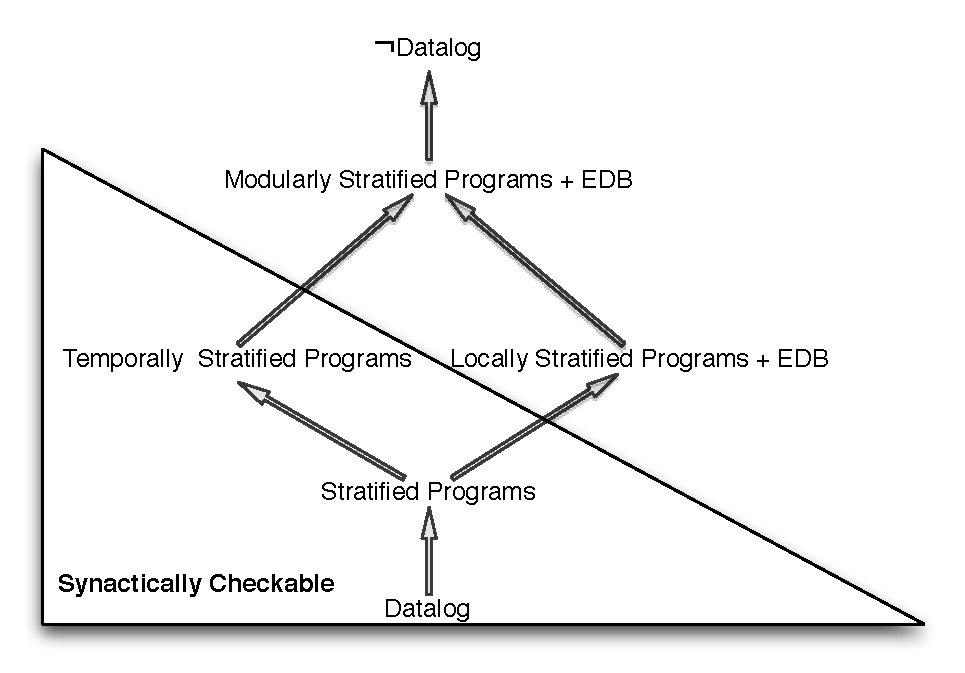
\includegraphics[width=0.75\linewidth]{figures/dedalus_classes.pdf}
  \label{fig:dedalus-classes}
  \caption{Stratifiability classes.  $A \to B$ means that every program in $A$ is in $B$.}
\vspace{-8pt}
\end{figure}


%%\paa{I don't think we can show that programs with async rules are locally stratifiable, actually}
%%\wrm{Why not?  What if we have that "causality constraint" we were talking about?}



\subsection{Temporal Safety}
Next we consider the issue of infinite results raised in the introduction to this section.
In traditional Datalog, this is a well-studied concern.
A Datalog program is considered {\em safe} if it has a finite minimal model, and hence has
a finite execution.  Safety in Datalog is traditionally ensured
through the following syntactic constraints:

\begin{enumerate}
%
\item No functions are allowed.
%
\item Variables are \emph{range restricted}: all attributes of the head goal
appear in a non-negated body subgoal.
%
\item The EDB is finite.
%
\end{enumerate}

These constraints ensure that the Herbrand Universe is finite: any atom that
may be deduced by a safe program may only take its attributes from the 
set of all constant symbols appearing in the program and EDB\@.
%%~\nrc{Don't know what this means, but I suspect it is fancy-pants language for no good reason.}
%%\paa{ignoring this provocative comment.}
%%\wrm{lol.}
In fact, the set of all possible assignments of these constants to predicate
attributes, representing every possible interpretation, is itself finite. 

Since our definition of \dedalus{successor} violates these rules, and indeed
leads to an infinite set of facts, \slang programs violate this
definition of safety.  However, \dedalus{successor} models time, not computation;
later sections explain how \lang implementations avoid enumerating the contents
of \dedalus{successor} at runtime.
%%\wrm{whats pailiative (helping fix the problem) here???}.  
This section
introduces a notion of termination that allows us to reason about the safety of
\slang programs.

%\nrc{Seems like there ought to be more here. Why do I care about the
%  preceding text? What does it have to do with the following text?}

%Since the Herbrand Universe is finite, any instantiation of predicates with
%constants is finite.  Every possible interpretation (set of ground atoms) of
%a logic program comes from this finite instantiation, so any possible
%interpretation is finite
  
%\paa{the idea is: safe=finite.  herbrand universe=finite, so any instantiation of predicates with constants is finite.
%every possible interpretation (set of atoms) of a LP comes from this instantition.  so any possible interpretation is finite.
%a model is an interpretation in which all heads are true when the body is true.  all models are finite.  the minimal model
%is clearly finite.}

%\subsection{Temporal Safety}

%%\wrm{show some examples before restricting to temporal safety!!  maybe even
%%show that some unsafe programs have safe equivalents.}

A \slang program containing only deductive rules is informally equivalent to a
Datalog program in which all predicates have no time suffix.  If all the rules
in such a program meet the conditions above, then clearly we would like them to meet \slang's definition of safety. 
%%\rcs{this used to say conditions 1 and 2, but it is possible that our program is infinitely long...  Also, ``clearly they are safe'' is strange, given that we haven't defined 
%%safety yet, so I reworded.}



\begin{definition}
%
A rule is \emph{instantaneously safe} if it is deductive,  function-free and range-restricted.
A \slang program is instantaneously safe if its deductive reduction is instantaneously safe.
%
\end{definition}

%Inductive rules may be unsafe.  Consider the \dedalus{successor} relation described above.  According to our
%intuitive interpretation, this relation models the passage of time, in order to
%establish a temporal order among ground atoms. 

The \dedalus{successor} relation complicates the discussion of safety, as it
introduces the countably infinite set $\mathbb{Z}$ to our
%Herbrand
universe of constants.
%Clearly, a naive interpretation of time can lead to unsafe programs:
%\rcs{how is this any more unsafe than succ(x+1) :- succ(x)?  Suggested text:}

%The infinte \dedalus{successor} relation complicates our discussion of safety;
Consider the following \slang program, which derives a single, persistent fact:

%Consider the \dedalus{successor} relation described above.  According to our
%intuitive interpretation, this relation models the passage of time, in order to
%establish a temporal order among ground atoms. 
%%\wrm{we're ignoring entanglement here}
%Recall that {\em successor} is the standard strict total order on
%$\mathbb{Z}$, lol, don't know how I accidentally wrote the above incorrect
%sentence all over the paper
%Recall that \dedalus{successor} is an infinite relation.  Clearly, a naive
%interpretation of time can lead to unsafe programs:

%%No reason to re-define a strict total order here...
%\begin{itemize}

%\item $\forall A,B \in \mathbb{Z} : successor(A, B) \Rightarrow B > A$ (i.e. whenever $successor(A,B)$ is true, then $B > A$)

%\item $\forall A \in \mathbb{Z} : \exists! B \in \mathbb{Z} : successor(A,B)$ (i.e. every integer has a successor)

%\end{itemize}

%\wrm{we'd expect a lot more properties of successor than the ones you mentioned.  so instead of trying to think of them all, i just narrowed down what you wrote.}

%This implies that successor is infinite (as we'd expect time to be), and is problematic because it leads to unsafe programs.


\begin{example}
\label{ex:tempsafe}
%
An unsafe \slang instance?
\\
%%\begin{Dedalus}
%%p\pos(A, B)@next \(\leftarrow\) p\pos(A, B), \(\lnot\)p\nega(A, B);
%%\end{Dedalus}
\begin{Dedalus}
persist[p, p\_neg 2]
p(1, 2)@123;
\end{Dedalus}

%%\paa{we shouldn't \emph{ever} need to write out r2, right?}

The single ground fact will cause one deduction for each tuple in
\dedalus{successor}.  Since \dedalus{successor} is infinite, the corresponding
Datalog
%%\rcs{what should we call this?}
program is unsafe.  
%
\end{example}

However, observe that each of these deductions produces a tuple that changes
only in its time suffix.  We find it useful to distinguish between unsafe
programs and programs that, given a finite EDB, eventually derive only tuples
that are equivalent except in their time suffixes.

%%\wrm{$<$don't really get whats going on$>$}
%%Consider a \emph{derivation tree} as defined by Levy et al~\cite{levy}.  
%%\paa{he's halevy now.  should it be halevy et al?  or is that confusing?  I blame alon.}
%%According to their definition,
%%two goal nodes $g_1$ and $g_2$ are \emph{identical} if they have the same predicate symbol and, in each argument
%%position, the same variables.  Two nodes are \emph{equivalent} if there exists a one-to-one mapping
%%$\phi$ from $V(g_1) \to V(g_2)$ such that $\phi(g_1) = g_2$.


%%\paa{I may have made a mess of this.  derivation trees are probably more machinery than we need to describe, for
%%the purposes of the definition of a 'stable inference', the 1-step deduction of an atom from another atom having the same
%%name and the same values for all attributes but time}
%%\wrm{I still don't know why we need to use derivation trees here.}
%%\wrm{Define 'derivation'.  Joe sez: "Here I think you just need an appropriate reference for derivation trees, along with some simple intuition.  I believe the right ref is %%"Constraints and Redundancy in Datalog", Levy/Sagiv, PODS 92."}

%%\begin{definition}
%%An \emph{inference} is a single step in a derivation, corresponding to a goal node, its child rule node, and the child goal
%%nodes of this rule node.  
%%\end{definition}

%%\paa{or... ditch all this stuff about derivations, define an 'inference' as a single deduction of an atom from established atoms;
%%ie the single evaluation of a rule, and proceed from here with the definitions}

%%\textbf{alternate derivation-free definition:}
%%\begin{definition}
%%An \emph{inference} is the deduction of an atom from established atoms via the application of a rule.
%%\end{definition}
%%\wrm{what's a rule application?}

%%\begin{definition}
%%A \emph{stable inference} has a goal $\gamma'$ with time suffix $\Tau$ derived
%%from a child goal $\gamma$ with time suffix $\Tau-1$, such that $\gamma$ differs from
%%$\gamma'$ only in its time suffix.
%
%%\end{definition}

%%In other words, $\pi_\xi(\gamma')$ is equivalent to $\pi_\xi(\gamma)$, where $\xi$ is the set of attributes in $\gamma$
%%minus $\Tau$.\wrm{$<$/dont really get whats going on$>$}.

%%\wrm{How about we delete everything above and just say this:}

%%To distinguish between programs that 
%%produce these infinite \emph{void inductions} and those that correspond 
%%intuitively to the Datalog notion of unsafe programs, we introduce the concept of
%%\emph{temporal safety}.

%%\begin{definition}
%%An intensional predicate $e$ in a program $P$ is called an \emph{event predicate} if there exist
%%in $P$ no rules with $e$ in their head. \wrm{how is this different from an EDB predicate??}
%%\end{definition}

\begin{definition}
%
Two sets of ground atoms $\Gamma$ and $\Gamma'$ are \emph{equivalent modulo
time} if each atom $\gamma \in \Gamma$ has a corresponding atom $\gamma' \in
\Gamma'$ such that $\gamma$ and $\gamma'$ have the same predicate symbol, and
the same assignment of constants to attributes for all attributes except the
time suffix.
%
\end{definition}

%%In other words, $\pi_\xi(\gamma')$ is equivalent to $\pi_\xi(\gamma)$, where $\xi$ is the set of attributes in $\gamma$
%%minus $\Tau$.\rcs{either define pi, write out ``projection'', or drop this paragraph}

\begin{definition}
%
We say a \slang instance is \emph{quiescent at time $T$} if the set of all
atoms with time suffix $T$ is equivalent modulo time to the set of all atoms
with time suffix $T-1$.
%%\rcs{what is a true atom?  Why distinguish between true atoms and false atoms?  Surely the neg tuples will match as well.  If not, then the program has somehow not quiesced...}
\end{definition}

%%\paa{well, there are some problems with this.  first, facts are only in the EDB, you mean atom,
%%second, this is never true because of the time suffix (unless you mean to have defined ``fact''
%%precisely as $\pi_\xi(p)$ for any predicate p.)  what I was trying to do was define quiescence in terms
%%of inference; a quiescent DB is one for which all inferences are stable.}

\begin{observation}
%
A \slang instance that is quiescent at time $T$ will be quiescent until
timestamp of the next EDB fact $V$, i.e.\ for all $U \in \mathbb{Z}: V > U >=
T$.  If no EDB fact has a timestamp greater than $T$, then the instance will be
henceforth quiescent.
%%\rcs{what does it mean for an edb fact to be true at time $T$?  It would be better to say that there is no EDB fact with timestamp T, since we're trying to ground the discussion without talking about time.}
%
\end{observation}
%
\begin{proof}
%
%%\wrm{sightly ???}
A \slang program admits only instantaneous and inductive rules, which derive
new tuples at the same time as their ground tuples, or in the immediate next
timestep.  Thus, the set of tuples true at time $T$ is completely determined by
any tuples true at time $T-1$, and any EDB facts true at time $T$.  Observe
that the integer value of the timestep does not influence the derivation.

If the instance is quiescent at $T$, then given ${\bf A}$, the set of atoms
with timestamp $T-1$, and the EDB at $T$, the program entails ${\bf
A}$ at timestamp $T$.  Thus in the absence of EDB facts at $T+1$, it entails
${\bf A}$ at $T+1$.
%
\end{proof}

\begin{definition}
%
A \slang instance with finite EDB is \emph{temporally safe} if it is henceforth
quiescent after some time $T$.
%
\end{definition}
%%\wrm{the following doesn't seem like a definition, seems more like a test for temporal safety}
%%\begin{definition}

\begin{definition}
%
Given the depends-on relation $\succ$ and its transitive closure $\succ^{*}$,
an intensional predicate $e$ in a program $P$ is called an \emph{instantaneous
predicate} if for every predicate $p$ for which $e \succ^{*} p$ (ie, $e$
depends transitively on $p$), either $p$ appears in the head of no inductive rules, or the body
of each inductive rule with head $p$  contains at least one positive instantaneous 
predicate.

\end{definition}

%%A rule is temporally safe if:
We propose the following conservative test for temporal safety.  A program is
guaranteed to be temporally safe if every rule is either:

\begin{enumerate}
%
\item An instantaneously safe rule, or
%
\item An inductive rule in which the head predicate occurs also in the
body with the same variable bindings for all attributes save the time suffix,
or
%%occurs also in the body with the same assignment of variables and constants to attributes.
%
\item An inductive rule that has at least one instantaneous predicate as a
positive subgoal in the body.
%
\end{enumerate}

%%\paa{maybe this is too greedy.  rule 1 above defines "instantaneous safety" or classical datalog-type safety.  
%%if all deductive rules respect rule 1, we are instantaneously finite.  the other two rules describe temporal safety
%%as such.  that is to say: any deductive rule that is range-restricted and function-free is instantaneously safe (deductive rules do
%%not reference the infinite relation \emph{successor}.  instantaneously safe <=> safe in datalog) further, any instantaneously safe rule is temporally safe.  
%%also, rules that are (2,3) are temporally safe.}

While a temporally safe program is henceforth quiescent after some time $T$,
a temporally unsafe program changes infinitely.  Note that
the \slang program in Example~\ref{ex:tempsafe} is temporally safe because
\emph{r1} satisfies the second condition above.

\begin{lemma} 
%
A temporally stratifiable \slang instance is temporally safe if it has a finite EDB and every rule is one of the kinds 1-3 above.
%
\end{lemma}
%
\begin{proof}
%
Assume the program is temporally unsafe.  That is, there exists no time $T$
such that $\forall U >= T$, the set of all atoms with timestamp $U$ is
equivalent modulo time to the set of all atoms with timestamp $T-1$.  Let $E$
be the maximum timestamp of any fact in the EDB.

Observe that every rule $r$ of kind 3 may only entail a finite number
of facts---as the EDB is finite---and thus may entail no facts at a
timestamp greater than some maximum timestamp $V_r <= E+1 \in
\mathbb{Z}$.  Since a \slang program has a finite set of rules we know
$\exists V \in \mathbb{Z} : \forall r: V >= V_r$, and thus $V <= E+1$.

We now consider times $T$ such that $T > E+1$.  By the above argument, no rules
of kind 3 entail any facts with a timestamp greater than $E+1$.  Recall that
no EDB atoms are true at any timestamp greater than $E$.  Thus, any facts with
timestamp greater than $E+1$ are entailed by rules of kind 1 or 2.

Consider the set of equivalence classes modulo time of all possible atoms, {\bf
A}, given the Herbrand universe.  We know {\bf A} is finite, as the Herbrand
Universe is finite.  Therefore, if the program is temporally unsafe, then {\bf B}, the
set of atoms entailed by the program, both contains and excludes
infinitely many members of at least one equivalence class in {\bf A} (i.e.,
something ``infinitely oscillates in time'' between being true and false).
Since the program has finitely many rules, at least one rule must entail
infinitely many atoms (from at least one of the equivalence classes from {\bf
A}). Thus, it is easy to see that there must be a cycle that contains some predicate $P$ and $\lnot P$.

We show there exists such a cycle containing only rules of kind 1, which
implies that the program is temporally unstratifiable.  In order for such a
cycle to exist, $P$ must transitively depend on $\lnot P$, and $\lnot P$ must
transitively depend on $P$.  Thus, the program contains a rule $J_1$ with
$\lnot P$ in its body, and some predicate $R$ in its head, as well as a rule
$J_2$ that is transitively dependent on $R$, with $P$ in its head.

{\bf Case 1: }$P \neq R$.  In this case, $J_1$ must be of kind 1, as for any $Q
\neq P$, a rule of kind 2 with $P$ in the head may not directly entail $Q$
given $P$.  $J_2$ must also be of kind 1---if it is of kind 2, then it
necessarily contains $P$ in its body, so it cannot entail $P$ unless $P$ is
entailed by some other rule.  If $J_2$ contains $R$ in its body, then the
program is syntactically unstratifiable.  But if $J_2$ does not contain $R$ in
its body, then it contains some predicate $S$ transitively entailed by $R$;
wlog the body contains $R$.  Thus, the program is syntactically unstratifiable.

{\bf Case 2: }$P = R$.  In this case, $J_1$ and $J_2$ are the same rule: $P
\leftarrow \lnot P$.  Thus, the program is syntactically unstratifiable.

Thus, the program is temporally unstratifiable, which contradicts our
assumption.
%
\end{proof}

\begin{example}
A \slang instance with a temporally unsafe deductive rule.
%%\rcs{is this even a \slang instance?  Is it a Datalog instance?  Perhaps this example belongs earlier in the text, where we define range-restricted.}


\begin{Dedalus}
p(A, B) \(\leftarrow\) q(A);
\end{Dedalus}

The program above has a temporally unsafe deductive rule that corresponds to an
unsafe rule in Datalog: it is not range-restricted.  The head variable $B$
could range over an infinite set of constants.
\end{example}


\begin{example} 
%
A \slang instance that is temporally unsafe due to infinite oscillation.

\begin{Dedalus}
flip\_flop(B, A)@next \(\leftarrow\) flip\_flop(A, B);
flip\_flop(0, 1)@1;
\end{Dedalus}

The above program exemplifies temporally unsafe induction. Even though it
contains no function symbols, and all variables are range-restricted, it
entails infinite oscillation of the \emph{p} predicate.  
%because the \emph{p} predicate occurs in the head with a different variable
%binding than in the body, and because there are no positive event predicates
%in the body.  
%%\wrm{this makes me a bit uncomfortable.
%%we've defined a conservative test for temporal safety.  so if something fails
%%the test, it's not necessariliy temporally unsafe.}
\end{example}

We can imagine interesting examples of temporally unsafe programs, and do not forbid them
in \slang. 
%%\wrm{joe sez "discuss safety is wil, but-out regured"}

%%By providing a conservative syntactic check for temporal safety, we ensure that \slang
%%programs have 

%An inductive rule cannot cause infinite oscillation if it has a positive event predicate in its body, because we are assuming a finite EDB.

%%However, we observe that all of these deductions are uninteresting, as they are
%%deterministically related to the EDB.  To avoid performing such deductions, we
%%restrict {\em successor} to range over the subset of $\mathbb{Z}$ consisting of
%%the consecutive natural numbers between the minimum and maximum timestamp
%%specified in the (finite) EDB ($\{123, 124\}$ in this example) \wrm{this is without NDB right?}.  If we extended the EDB with the additional facts:

%But if \emph{successor} is infinite, many of these deductions may be \emph{void}in some sense, i.e. functionally determined based on the EDB. \wrm{is functionally determined a real term?}
%In effect, an EDB that is given in its totality determines a window over successor that is relevant to any computation that must be performed.  \wrm{what about NDB?}
%It is easy to see that in this example, we need only consider a successor relation that contains a single tuple \{123, 124\}.

%%\begin{Dedalus}
%%delete p(1, 2)@456;
%%p(?, ?)@789; \wrm{we're still doing queries?}
%%\end{Dedalus}

%%Evaluating the \lang instance would require \emph{successor} to range over the
%%subset of consecutive natural numbers $[123, 790]$.

%%\begin{definition}
%%A \emph{post-hoc} evaluation is an evaluation of a \lang instance where
%%{\em successor} ranges over the finite subset of $\mathbb{Z}$ described above.
%%\end{definition}

%%In a post-hoc evaluation, we can derive {\em successor} from the EDB as part of
%%the fixpoint computation.  We first define a predicate \emph{event\_time} that
%%contains the union of the time attributes from the EDB:

%%$event\_time(\Tau) \leftarrow \displaystyle\bigvee_{p \in EDB} p([...], \Tau)$

%%\wrm{I wasn't a fan of expressing a query plan in a Datalog rule...  But we can
%%talk about this}

%%We then populate \emph{successor} with \lang program shown below:
%with arithmetic and aggregate functions, as shown below.

%%\begin{Dedalus}
%%smax(max<N>) \(\leftarrow\) event\_time(N);
%%smin(min<N>) \(\leftarrow\) event\_time(N);

%%successor(N, N + 1) \(\leftarrow\) smin(N);

%%successor(S, S + 1) \(\leftarrow\) 
%%    successor(N, S),
%%    smax(M),
%%    N <= M;
%%\end{Dedalus}

%%\wrm{Not sure what the point of this is...}
%%Since {\em successor} is finite in a post-hoc evaluation, we may evaluate the
%%ntire \lang instance in a single fixpoint.

%In a post-hoc evaluation, time is in some sense ``instantaneous" in that all values of the successor relation are considered in a single
%fixpoint computation.  The complete program is safe if the EDB is finite.


